\documentclass[crop,tikz]{standalone}
\usepackage{tikz}
\usetikzlibrary{trees, positioning, arrows.meta}

\begin{document}

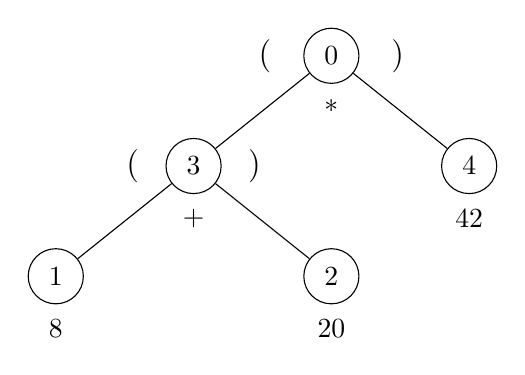
\begin{tikzpicture}[
  level distance=14mm,
  sibling distance=35mm,
  opnode/.style={circle, draw, minimum size=7mm},
  leaf/.style={circle, draw, minimum size=7mm},
  paren/.style={font=\large}
]

% -------------------------
% Tree structure (NO labels in operator nodes)
% -------------------------

\node[opnode] (mul) {0}
  child {
    node[opnode] (plus) {3}
      child { node[leaf] (n8) {1} }
      child { node[leaf] (n20) {2} }
  }
  child { node[leaf] (n42) {4} };

% -------------------------
% Operator labels UNDER nodes
% -------------------------

\node[below=2pt of mul]  {$*$};
\node[below=2pt of plus] {$+$};
\node[below=2pt of n8] {$8$};
\node[below=2pt of n20] {$20$};
\node[below=2pt of n42] {$42$};

% -------------------------
% Parentheses (outside operator nodes)
% -------------------------

% Around plus subtree
\node[paren, left=6pt of plus] {(};
\node[paren, right=6pt of plus] {)};

% Around full expression (mul root)
\node[paren, left=8pt of mul] {(};
\node[paren, right=8pt of mul] {)};

\end{tikzpicture}

\end{document}
